\chapter{Physics Beyond the Standard Model}
\label{ch:theory}
In light of the various phenomenon unexplained by the Standard Model, physicists have proposed various extensions to the Standard Model, collectively termed \textit{Beyond the Standard Model} (BSM) theories. 
A particular focus of the physics programs at the Large Hadron Collider (LHC) are BSM models which suggest dark matter candidate particles. If these particles couple to Standard Model, they could be produced and observed at the LHC.
This chapter will explore Hidden Valley models, and in particular the potential for Hidden Valley models to produce \textit{semi-visible jets}. This will set the theoretical foundations for the experimental search presented in the later chapters of this thesis. The mechanisms of dark QCD that arise from these models and allow for the production of semi-visble jets will also be discussed.

\section{Hidden Valley Models}
\label{sec:hiddenvalley}

Hidden Valley (HV) models are a category of BSM models that allow for dark matter (DM) production at the LHC. They extend the Standard Model with an additional non-Abelian gauge group \cite{snowmass}. This introduces the possibility of a complex dark sector, which mirrors the complexities of Standard Model QCD, and introduces the possibility of dark quarks and gluons. The term ``hidden valley" refers to the idea that the DM is hidden from the SM by a high-energy barrier, as illustrated in Figure~\ref{fig:hidden_valley_sketch}. The dark sector is assumed to communicate with the Standard Model via a ``portal", or ``messenger particle", that can interact with both Standard Model and HV forces. For the s-channel scenario, the portal is considered to be a new massive mediator particle $Z'$ . \par

\begin{figure}[h]
        \centering
	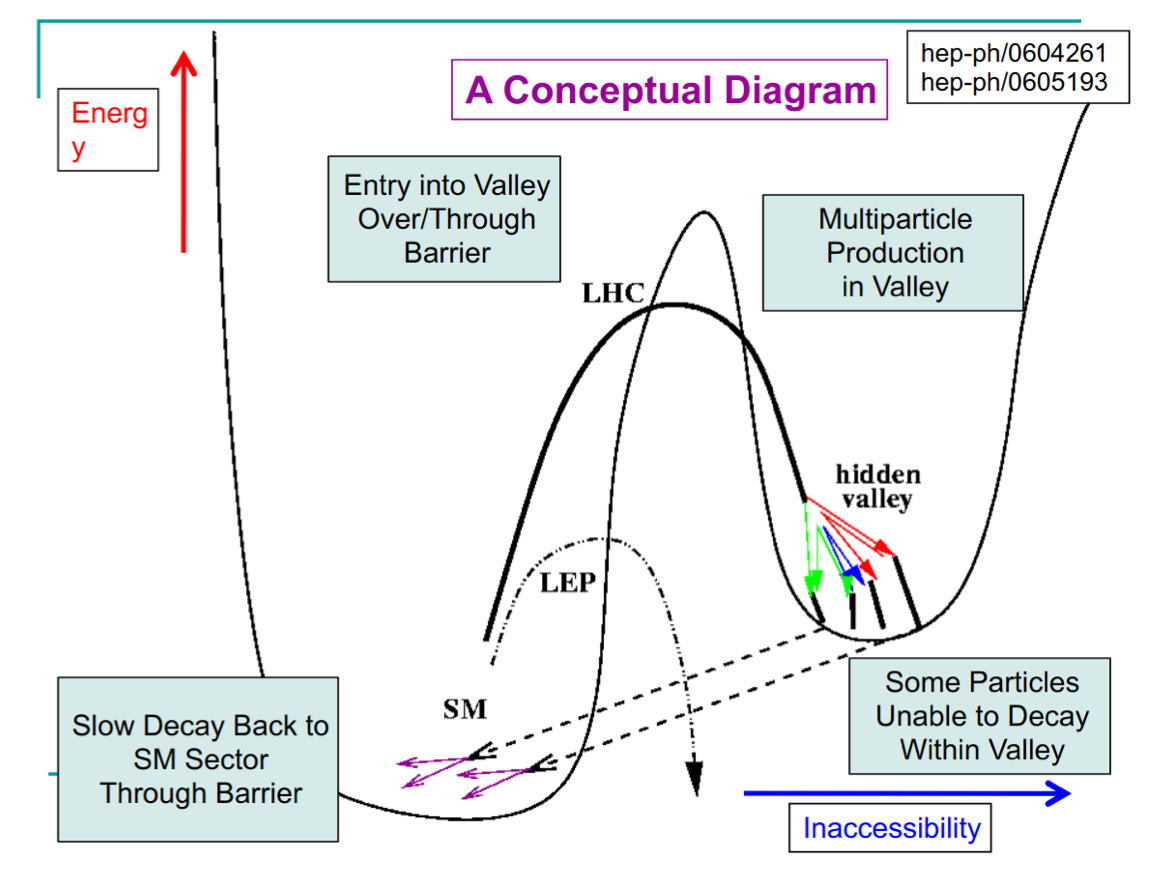
\includegraphics[width=.5\textwidth]{figures/ch2/hidden_valley_sketch.png}
         \caption{Illustration of the hidden valley potential.
         \label{fig:hidden_valley_sketch}}
\end{figure}

The portal particle allows for the production of dark sector particles at hadron colliders. If dark quarks are produced via the decay $Z' \rightarrow q_D \bar{q_D}$ they can hadronize and form dark jets. The properties of the dark jets are determined by the dynamics of the dark sector, which are explored in the subsequent section. Depending on the details of the model, the jets formed by the dark hadrons can be categorized as fully dark, semi-visible, leptonic, emerging, or other \cite{snowmass}. \par

\begin{figure}[h]
        \centering
	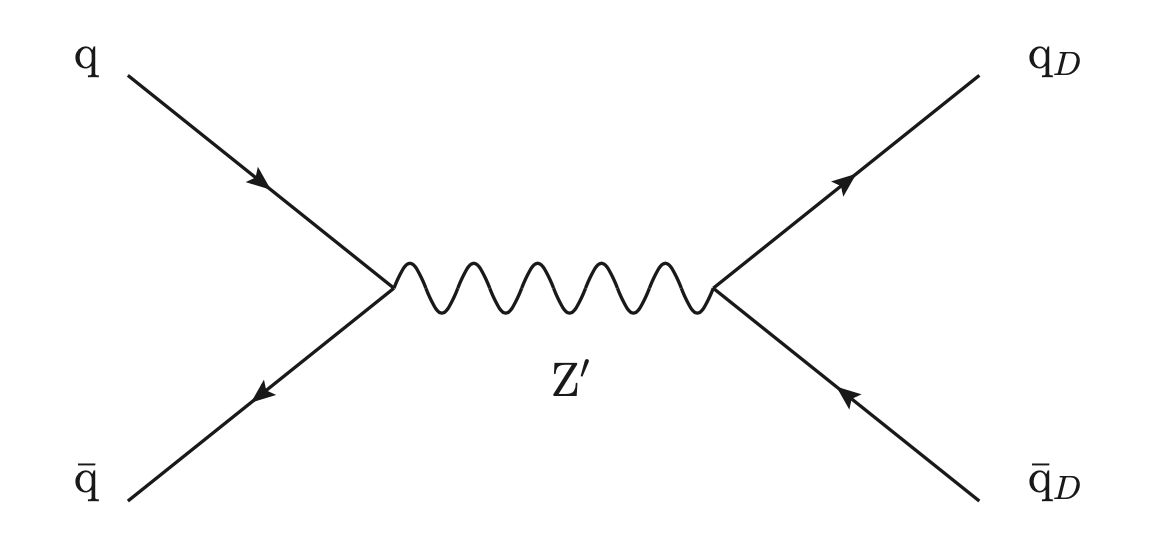
\includegraphics[width=.5\textwidth]{figures/ch2/zprime_feynman_diagram.png}
        \label{fig:ch2/zprime_feynman_diagram.png}
        \caption{The massive mediator particle $Z'$ of the s-channel realization of a HV model}
\end{figure}

\section{Dark QCD}
\label{sec:darkqcd}
The theoretical underpinning of the semi-visible jet phenomenology is a dark sector with a gauge group $SU(N)_d$ leading to confinement at a scale $\Lambda_d$. For illustration, let's consider the case of an $SU(2)_d$ gauge theory, which gives rise to two dark fermionic generations $\chi_a = \chi_1, \chi_2$. Following the work of Ref.~\cite{darkqcd} we can write the fundamental dark Lagrangian as:
\begin{equation}
	\mathcal{L}_{dark} \supset - \frac{1}{2} \Tr G^{d}_{\mu\nu} G^{d\mu\nu} - \bar{\chi_a} (i {D\mkern-11.5mu/}-M_{d,a}) \chi_a
\end{equation}

The first term allows for the dark gluons to self-interact, while the second term enables the dark quarks to hadronize and acquire mass. The dark quarks are assumed to have a common mass $M_d$. The coupling strength of the strongly interacting dark quarks is termed $\alpha_d$. At the confinement scale $\Lambda_d$, the dark quarks can form bound states. At the scale $M_d \approx \Lambda_d$ a QCD-like shower occurs. \par 

The properties of the hadrons formed by the dark quarks are of particular importance to the observed dark QCD dynamics. Dark-isospin number $U(1)_{1-2}$ and dark-baryon number $U(1)_{1+2}$ are accidental symmetries of the theory which determine the stability of the hadrons. In the case of two dark flavors, six dark hadrons can be formed: four mesons ($\chi_1\bar{\chi_1}$, $\chi_2\bar{\chi_2}$, $\chi_1\bar{\chi_2}$, $\bar{\chi_1}\chi_2$) and two baryons ($\bar{\chi_1}\bar{\chi_2}$, $\bar{\chi_1}\bar{\chi_2}$). The mesons $\chi_1\bar{\chi_2}$ and $\bar{\chi_1}\chi_2$ are charged under dark-isospin and will be stable if this symmetry is unbroken. The baryons would also be stable as they are charged under the dark-baryon number. These four stable hadrons become dark matter candidates of the theory. The $\chi_1\bar{\chi_1}$ and $\chi_2\bar{\chi_2}$ mesons are not charged under either symmetry and are thus expected to decay. The unstable mesons can decay into stable dark mesons, or into an off-shell $Z'$. The off-shell $Z'$ will then decay into two DM quarks or two SM quarks, and its products will continue to shower until the final state particles are stable.\par

The number of stable and unstable dark states varies substantially depending on the details of the model. The model discussed above can be generalized from $SU(2)_d$ to $SU(N)_d$, with any number of colors $N_c$ or flavors $N_f$. This affects the ratio of possible stable to unstable mesons, which can directly impact the amount of missing energy. The fraction of missing energy is a variable in many dark QCD models, and is especially important in the case of semi-visible jets.

\section{Semi-visible Jets}
\label{sec:semivisiblejets}

A ``semi-visible jet'' occurs when the heavy $Z'$ messenger particle decays into dark quarks, which then hadronize in a QCD-like shower. If some of the dark hadrons are stable while others decay to SM quarks via the off-shell $Z'$, a collimated mixture of visible and dark matter is formed – this is termed a semi-visible jet. If the $Z'$ messenger particle is produced at rest, the two jets will be back-to-back in the transverse plane. If there is an imbalance in the amount of invisible particles between the two jets, one of the jets will be observed to be aligned with missing transverse energy. \par

While there are a myriad of HV and dark QCD models, a handful of model parameters are most important in determining the observable of these showers within a particle detector. The coupling strength $\alpha_d$ is one of the most important, as it controls the fraction of dark hadrons emitted in the shower and their average \pt. The mass of the dark quarks directly impacts the jet mass. If the masses of the dark quark flavors are comparable, the ratio of stable to unstable dark hadrons will be approximately 1:1. However, if there is a mass splitting, stable or unstable dark hadrons may be favored, which impacts the amount of missing energy observed. \par

The ratio of stable to unstable dark hadrons in the shower is a critical variable for capturing the behavior of dark showers. This value is termed \rinv:
\begin{equation}
	R_{inv} = \frac{\textrm{\# of stable hadrons}}{\textrm{\# of hadrons}}
\end{equation}

Events containing jets aligned with missing transverse momentum are generally considered to be misreconstructed by other DM searches, and therefore discarded. This class of final states is therefore largely uncovered by existing DM searches. The nature of the dark hadron shower is determined by the following parameters: the $Z'$ mass $m_{Z'}$, the $Z'$ couplings to visible and dark quarks $g_q$ and $g_{q_D}$, the number of dark colors and flavors, the characteristic scale of the dark sector confinement $\Lambda_D$, the mass scale of the dark hadrons $m_D$, and the average fraction of stable hadrons in the decay \rinv. The coupling to SM quarks determines the $Z'$ production cross section.

